\documentclass[10pt, conference, letterpaper]{IEEEtran}
\usepackage{cite}
\usepackage{xcolor,soul,framed}
\usepackage{amsmath,amssymb,amsfonts}
\usepackage{algorithmic}
\usepackage{graphicx}
\usepackage{color, soul}
\usepackage{svg}
\graphicspath{ {./images/} }

%---------------------------------------------------------------%
%-Include Graphics Macro:---------------------------------------%
% \begin{figure}[h]                                             %
%     \centering                                                %
%     \includegraphics[width=0.45\textwidth]{*}                 %
%     \caption{}                                                %
%     \label{fig:*}                                             %
% \end{figure}                                                  %
%-Include PDF Figures Macro:------------------------------------%
% \begin{figure}[h]                                             %
%     \centering                                                %
%     \includegraphics[width=0.45\textwidth, trim={0.5cm 0.5cm 0.5cm 0.5cm}, clip]{*.pdf}
%     \caption{}                                                %
%     \label{fig:*}                                             %
% \end{figure}                                                  %
%---------------------------------------------------------------%

\begin{document}

    %=============================== TITLE ===============================%
    \title{
        Meet-in-Future: Optimized Job Dispatching with Obsolete Information MDP in Edge Computing System
    }
    \author{
        \IEEEauthorblockN{HONG Yuncong}
        \IEEEauthorblockA{
            \textit{Department of CS}, The University of Hong Kong, China \\
            ychong@cs.hku.hk
        }
    }
    \maketitle

    %============================== ABSTRACT ==============================%
    \begin{abstract}
        \label{sec:abstract}
        We formulate the problem with job dispatching in distributed Edge Computing system, and identify the difficulty exists in cooperation between APs (Access Points) and ESs (Edge Servers) with delayed information. In this work, we design the broadcast information in the system and formulate the corresponding problem into two-time-scale MDP problem.
    \end{abstract}

    \begin{IEEEkeywords}
        Edge Computing, Distributed Scheduling, Delayed Information, Collective Observability, Distributed Multi-agent MDP
    \end{IEEEkeywords}

    %============================ INTRODUCTION ============================%
    \begin{section}{INTRODUCTION}
        \label{sec:introduction}
        (in progress)

        Some traits to mention compared to related works:
        \begin{itemize}
            \item we don't accept communication cost in broadcast, because the global information to share requires both collective information and delayed information and the waiting time for scheduling should be avoided.
        \end{itemize}
    \end{section}

    %========================= LITERATURE REVIEW ==========================%
    \begin{section}{LITERATURE REVIEW}
        \label{sec:review}
        \begin{itemize}
            \item We use MDP definition in \cite{sutton1998introduction}
            \item The earliest related works we find is \cite{ref-01} (cited 167 times). In this work, the single agent is assumed not able to observe the global state, and thus they need communication to establish cooperation by sharing \emph{information}. The agent considers communication as extra action to synchronize the states and thus incurs extra cost. \\
            However, the communication is without delay, and converted into POMDP problem.
            \item The other work \cite{ref-02} considers continuous state observation with constant or stochastic delay with single agent. \\
            However, 
        \end{itemize}
    \end{section}

    %============================ FORMULATION =============================%
    \begin{section}{FORMULATION}
        \label{sec:formulation}

        In this section, we will firstly give out the definition of job dispatching models in the edge computing system. Then we illustrate the definition of the proposed optimization problem, and formulate it under MDP framework. The formulated distributed problem assumes APs apply their action independently on observation of broadcast information from other nodes with a reasonable broadcast design, and thus forms a collection of obsolete global states consensus on a global utility function. At last, we also give out the global problem definition with respect to our problem for comparison as upper bound.

        \begin{subsection}{Model Definition}
            In a Mobile Edge Computing (MEC) system, the mobile users would offload their computation jobs to the selected APs (Access Points) to the Edge Computing network. The APs would make decisions on each jobs to determine which ES (Edge Server) could better serve it and then dispatch jobs to the corresponding ES with a certain delayed time.
            
            In our problem, we consider the process of jobs from release until be fully processed. We identify the \emph{response time} of this process is mainly composed of: waiting time on AP to make decision, uploading time from AP to ES, and total computation-and-waiting time on ES.
            The details about the communication model and computation model for jobs will be elaborated in the following subsection. Moreover, to facilitate the cooperation among multiple APs, the well-designed broadcast is also elaborated in this section to help APs come to consensus on global states.
            
            \begin{subsubsection}{Communication Model}
                The communication model in our system ignores the underlaid physical property and MAC design. We focus on the communication process of uploading of jobs.
                The assumed uploading time is deterministic and known in advance when the job is released to AP. The uploading time for one job may variance with respect to different ESs from the arrived AP, and the distribution of variance is not known in advance but is guaranteed with an expectation.
                Moreover, we assume the uploading process could be parallel among jobs which implies almost infinite capacity, and the end-to-end time is domain by the propagation time and processing time rather than communication time due to bandwidth. We identify this feature as the intrinsic property different from cloud computing scenario.
                
                When the dispatching action is going to applied from AP agent's view, all the AP and ES nodes need to broadcast their local jobs' information for cooperation. The broadcast delay is considered deterministic and asynchronous at their own pace.
                The details of broadcast design about interval and contents will be elaborated in the following \textit{Broadcast Model} subsection.
            \end{subsubsection}

            \begin{subsubsection}{Computation Model}
                We assume that there is only one job being computed at one time on the edge server. The computation model is assumed to be deterministic.
                Moreover, we assume unrelated parallel machine model which implies that the computation time for one job is known when released but has no relationship among the edge servers.
            \end{subsubsection}

            \begin{subsubsection}{Broadcast Model}
                \begin{itemize}
                    \item global aligned broadcast; interval is far larger than the maximum delay from one nodes to the other AP nodes;
                    \item consensus delay for $k$-th AP:
                        \begin{align}
                            \hat{d}_k = \max_{i\in(\mathcal{K} \cup \mathcal{N})}(d_{k,i})
                        \end{align}
                        and $\tau T + \hat{d}_k$ is the starting point of $\tau$-th stage for $k$-th AP;
                    \item Stage for $k$-th AP:
                        \begin{align}
                            (x_k={\tau})\triangleq t \in [\tau T^{br}+\hat{d}_k, (\tau+1) T^{br}+\hat{d}_k]
                        \end{align}
                        where $\tau$ is the general global state between $(\tau-1) T$-th and $\tau T$-th timeslot for all the AP nodes;
                    \item broadcast all of the information between the interval
                \end{itemize}

                The illustration figure \ref{fig:brd} for single broadcast includes several important time points which are also important in multiple synchronous broadcast: $x_{k,j}, d_{k,j}, T^{br}_{k,j}$
                \begin{figure}[h]
                    \centering
                    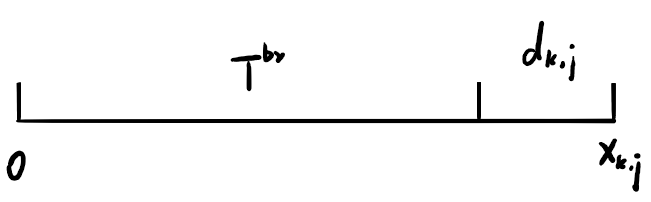
\includegraphics[width=0.45\textwidth]{single-broadcast.png}
                    \caption{Single broadcast timing illustration}
                    \label{fig:brd}
                \end{figure}
                And with the implication from the single broadcast, we generalize the conclusion for every broadcasts with:
                \begin{align}
                    x_{k,j} = d_{k,j} + T^{br}_{j}
                \end{align}
                which takes a reasonable assumption that $T>d$ always ($j=k',n$ for $k$-th AP).
            \end{subsubsection}
        \end{subsection}

        \begin{subsection}{Problem Formulation}
            In this section we will firstly give out our optimization utility under a reasonable definition of edge computing system. As we are also considering cooperation among AP agents via a delicate broadcast design, we furthermore express the control policy decentralized on each AP agent.
            By leveraging a delicate broadcast design, all the AP agents could receive the local features about jobs at the broadcast point and the experienced local cost (number of jobs) during the broadcast interval.
            We formulate the local MDP optimization processes with the same target as the global optimization utility, but all with delayed cost to collect and delayed actions to apply based on the obsolete observation via broadcast. However, due to the different broadcast delay for each agents, the agents come to the consensus global states at different timeslot and thus compose the states transition, which is different from the situation with updated global information on each agents. We will discuss the difference and optimality gap at the end of this section.

            \begin{figure}[h]
                \centering
                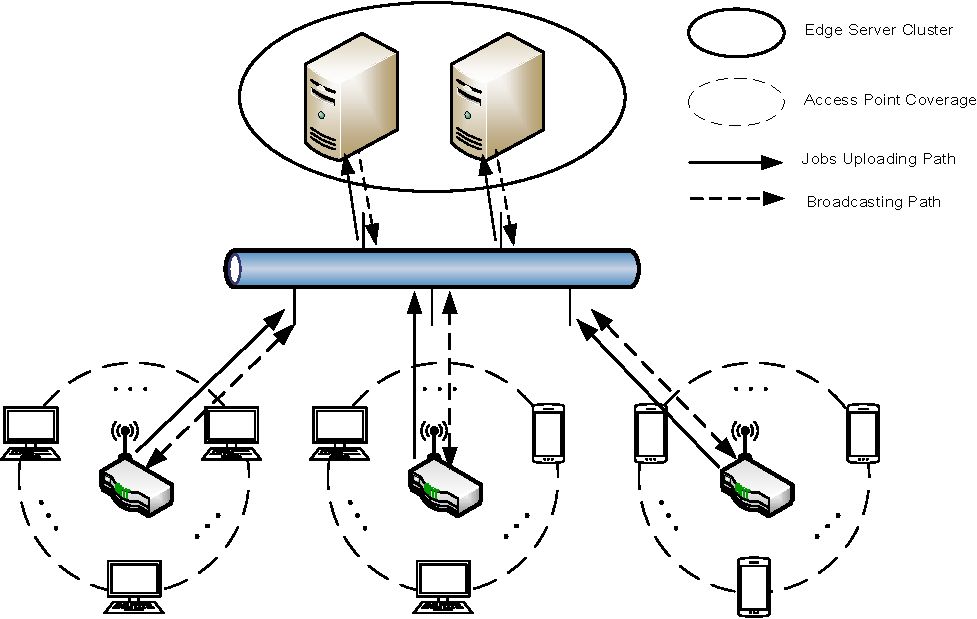
\includegraphics[width=0.45\textwidth, trim={0.5cm 0.5cm 0.5cm 0.5cm}, clip]{system-model.pdf}
                \caption{The Illustration of System Model}
                \label{fig:system}
            \end{figure}

            \begin{subsubsection}{Optimization Problem}
                We assume that there are $K$ APs and $N$ ESs in the MEC system.
                The arrival process of jobs at $k$-th AP is: $A^{(k)}(t)=I[t; L_C]$ which is a indicator random process. It will return $0$ if no jobs arrive at $t$-th time slot, and return the job with property $L_C$ if one job arrives, where $L_C$ is a vector of length $N$ denoting the deterministic computation time on unrelated machines.
                The computation time $L_C$ is bounded by $T_C$, i.e. $L_C \in [1,T_C]$.
                
                For one job $j$, it will wait until the uploading decision is made for it. Then it takes a general $T^{prop}_{k,n}$ time to be uploaded to $n$-th server from $k$-th access point; after being uploaded to $n$-th server, it will wait for its turn for computing until all the $L_C(n)$ components are processed and leave the system.
                
                Our optimization target is to minimize the average waiting time and computation time for each job, which is called the jobs' average response time. According to \emph{Little’s Law}, to minimize average response time, is equal to minimize the average number of jobs in a system, which is:
                \begin{gather}
                    \min_{\Omega} \lim_{T \to \infty} E[\frac{1}{T} \sum_{t=0}^{T} N(t)]
                    \\
                    N(t) = \sum_{k \in K} (A^{(k)}(t) + N_k(t))
                            + \sum_{n \in N} N_n(t)
                \end{gather}
                where $N_k(t)$ denotes the number of jobs on $k$-th AP, and $N_n(t)$ denotes the number of jobs on $n$-th ES.
                The goal to minimize the cost caused by ESs could be simply achieved with heuristic algorithm \emph{SJF} (shortest-job first), because it is the fastest way to reduce number of jobs on the edge server. So, in the next MDP problems we will focus on the policy applied on AP side, and leave ES with fixed heuristic algorithm.
            \end{subsubsection}

            \begin{subsubsection}{Single-Step Transition}
                We adapt the problem description at job-level grains and formulate the global states at $t$-th timeslot into job sets at APs and ESs:
                \begin{align}
                    S(t) \triangleq
                    \begin{Bmatrix}
                        S_{k}^{(W)}(t) = \{ (L_C) \}_{N_{k}^{(W)}}
                        \\
                        S_{k,n}^{(U)}(t)= \{ (L_C), L_{cd}^{(U)}(t) \}_{N_{k,n}^{(U)}}
                        \\
                        S_{n}^{(C)}(t)  = \{ L_{cd}^{(C)}(t) \}_{N_{n}^{(C)}}
                    \end{Bmatrix}
                    _{k\in\mathcal{K}, n\in\mathcal{N}}
                \end{align}
                where $L_C$ is a constant vector of length $N$ with each denoting the computation time of that job on each server; and $L^{(U)}_{cd}(t), L^{(C)}_{cd}(t)$ are countdowns for uploading and computing time remained for that job respectively.
            
                The single step transition graph is given below:
                \begin{figure}[h]
                    \centering
                    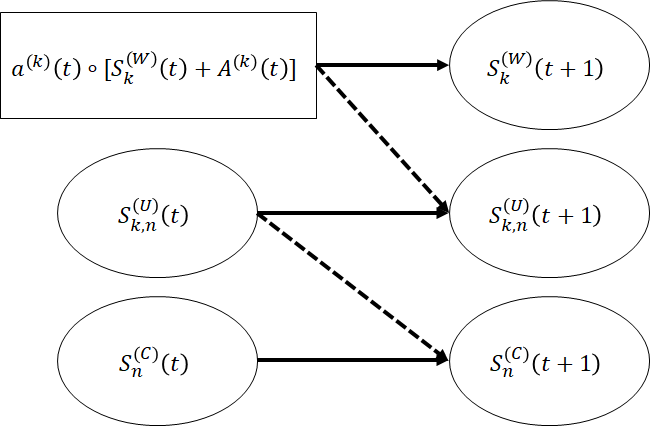
\includegraphics[width=0.45\textwidth]{single-transition.png}
                    \caption{Single-step transition function composing graph}
                    \label{fig:trans}
                \end{figure}
                \\
                Besides the states definition being illustrated above, we also have policy definition for $\vec{\Omega}(t) \triangleq (\Omega^{(1)}(t), \dots, \Omega^{(K)}(t))$ given the state $S(t)$. Each single policy $\Omega^{(k)}(t)$ defined on $k$-th AP is based on job-wise policy distribution $\vec{\alpha}^{(k)}$.

                The singleton action $a^{(k)}$ is defined for $k$-th AP as: for type-$j$ job, it should keep waiting or being uploaded to $n$-th server denoted as $\{0,1,\dots,N\}$. the action space is:
                \begin{align}
                    A \triangleq \{a|a \in Z_*^{N+1}\}
                \end{align}
                As we have total $L_C^{N}$ kinds of jobs for all the unrelated machine, we have the set $\mathcal{J}=\{1, \dots, L_C^{N}\}$ denoting the job type index and the singleton policy on singleton action related with $j \in \mathcal{J}$ is:
                \begin{align}
                    \vec{\alpha} \triangleq \{\alpha_1,\dots,\alpha_J\}
                \end{align}
                where $\alpha_j(a) \geq 0$ for all $a \in A$ and $\sum_a \alpha_j(a) = 1$.

                Then we give the denotations of a fixed job-wise policy distribution, which is called \emph{composed fixed policy} only related with $S^{(W)}(t), A^{(k)}(t)$ but not with the whole system features at $t$-th timeslot. The distribution for \emph{composed fixed policy} on $k$-th AP at $t$-th timeslot is given as:
                \begin{align}
                    \Omega^{(k)}(t) &= \Pr\{a^{(k)}(j), \forall j \in S^{'(W)}_k(t)\}
                    \nonumber\\
                    &= \prod_{j \in S^{'(W)}_k(t)} \alpha_{2^{L_C}}^{(k)}(a)
                \end{align}
                where $S^{'(W)}_k(t) \triangleq S^{(W)}_k(t) \cup A^{(k)}(t)$ and the decision on each job is based on the job type indexed with $2^{\vec{L_C}}$ and independent from each other. The output of this function gives the distribution of the \emph{joint uploading decision} of length $S^{'(W)}_k(t)$ on job set indexed with $\{1,\dots,|S^{'(W)}_k(t)|\}$.

                While the jobs processing is carried out following a descriptive procedure in the model section, we need some denotations to characterize the intrinsic of the transition. Firstly We come up with denotations for transition job sets expressed in figure \ref{fig:trans} as:
                \begin{align}
                    I^{(W \to W')}_{k}(t) & \triangleq \{ j | \vec{\alpha}_j(a=0), \forall j \in S^{'(W)}_k(t)\}
                    \\
                    I^{(W \to U)}_{k,n}(t) &\triangleq \{ j | \vec{\alpha}_j(a=n), \forall j \in S^{'(W)}_k(t)\}
                    \\
                    I^{(U \to C)}_{k,n}(t) &\triangleq \{j|(L^{(U)}_{cd})_j=1, \forall j \in S^{(U)}_{k,n}(t)\}
                    \\
                    I^{(U \to U')}_{k,n}(t) &\triangleq S^{(U)}_{k,n}(t) \backslash I^{(U \to C)}_{k,n}(t)
                    \\
                    I^{(C \to \Phi)}_{n}(t) &\triangleq \{j|\arg\min_{j} (L^{(C)}_{cd})_j \wedge (L^{(C)}_{cd})_j=1\}
                    \\
                    I^{(C \to C')}_{n}(t) &\triangleq S^{(C)}_{n}(t) \backslash I^{(C \to \Phi)}_{n}(t)
                \end{align}
                Then we establish the relationship between those indicator functions with $S(t+1)$:
                \begin{align}
                    \begin{cases}
                        S^{(W)}_{k}(t+1) = I^{(W \to W')}_{k}(t)
                        \\
                        S^{(U)}_{k,n}(t+1) = I^{(W \to U)}_{k,n}(t) + I^{(U \to U')}_{k,n}(t)
                        \\
                        S^{(C)}_{n}(t+1) = \sum_k I^{(U \to C)}_{k,n}(t) + I^{(C \to C')}_{n}(t)
                    \end{cases}
                \end{align}
                And we note that only $I^{(W \to W')}_{k}(t)$ and $I^{(W \to U)}_{k,n}(t)$ are affected from disturbance from arrival process and randomized policy. With $\Omega^{(k)}(t)$ and $A^{(k)}(t)$ determined, we could obtain the joint distribution of local states on $k$-th AP as:
                \begin{align}
                    & \Pr\{\begin{pmatrix}
                        S^{(W)}(t+1) \\ S^{(U)}(t+1)
                    \end{pmatrix}
                    |
                    \begin{pmatrix}
                        S^{(W)}(t) \\ S^{(U)}(t)
                    \end{pmatrix}, \vec{A}(t), \vec{\Omega}(t)
                    \}
                    \nonumber\\
                    = &\prod_{k \in K} \Pr\{ A^{(k)}(t) \} \times \Omega^{(k)}(t)
                \end{align}

                On the server's side, the states transition is easily to obtain because the computation process on server is totally deterministic between adjacent timeslots:
                \begin{align}
                    \Pr\{ S_{n}^{(C)}(t+1) |S_{n}^{(C)}(t), \{S_{k,n}^{(U)}(t)\}_{k \in \mathcal{K}} \} = 1
                \end{align}
                At last, we could come out with the global states transition function composed of the two parts as:
                \begin{align}
                    & \Pr\{ S(t+1)|S(t), \vec{A}(t), \vec{\Omega}(t)  \}
                    \nonumber\\
                    = & \prod_{k \in K} \Pr\{ A^{(k)}(t) \} \times \Omega^{(k)}(t)
                \end{align}
            \end{subsubsection}

            \begin{subsubsection}{Multi-Step Transition}
                We adapt aligned broadcast in practice where all of nodes will broadcast their local features at the point of broadcast and the cost collected in the broadcast interval.
                This joint information composes obsolete observations on all the AP nodes, and the nodes thus establish consensus on a global features. We assume that AP agents would take action on the one-step-backward obsolete observed states which result into a Markovian process and will be explained followed.

                We denote the collective global consensus observation on local features as:
                \begin{align*}
                    & S_0, S_1, S_2, S_3, \dots
                \end{align*}
                where $S_i \triangleq S(iT^{br})$. it stresses that each agent all maintains the same $S_i$ for a $T^{br}$ period but not aligned due to different consensus delay $\hat{d}_k$ on each agent.

                In this consensus formulation which is illustrated in figure \ref{fig:br-trans}, we actually let every agents know the global states with different deterministic delay. The delayed information doesn't impact on global states formulation of MDP problem, but converted into delayed composed action. For example, the agent would take actions based both on global states $S_1$ and $S_2$ in the period of $S_3$, because in the first half period it doesn't come to consensus on global states $S_2$.

                \begin{figure}[h]
                    \centering
                    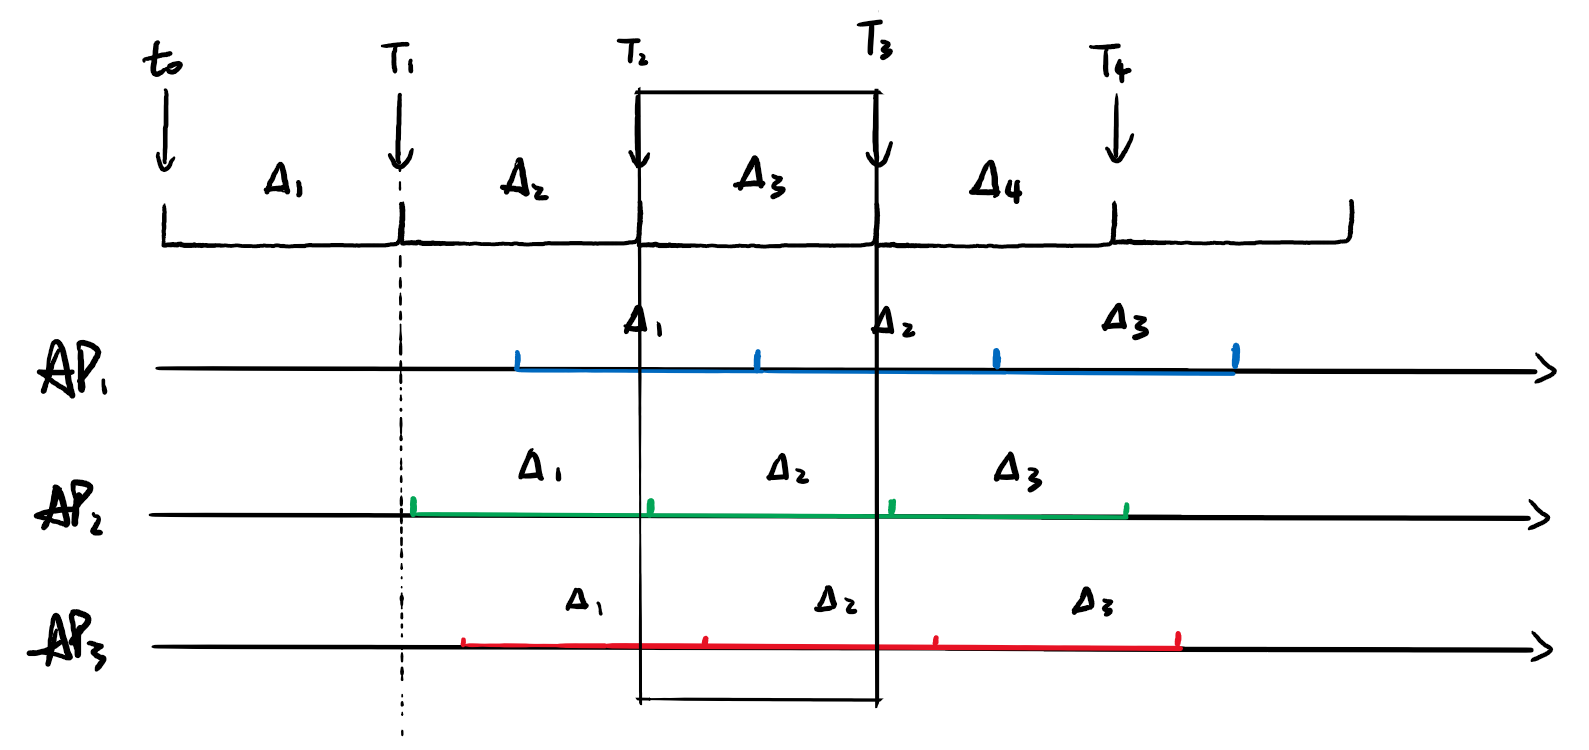
\includegraphics[width=0.45\textwidth]{broadcast-trans.png}
                    \caption{Global Consensus and Transition with Delayed Action}
                    \label{fig:br-trans}
                \end{figure}

                This implies that: \hl{The agents meet states in future with actions traced back into past}. The agents would contribute into global state transition, but the limited observation with obsolete information makes them always choose action based on the one-step-latter global states. So, one agent should carry out \emph{policy improvement} with other agents who fix their actions in its iteration. This improvement iteration comes to convergence always as the observations do not change with respect to policies.

                To formulate the transition between states, we firstly give out the denotation for single-step transition with fixed action given previous state $s$ as:
                \begin{align}
                    p(\vec{a}|s) \triangleq \Pr\{ S(t+1)|S(t)=s, \vec{\Omega}(\vec{a}),\vec{A}(t) \}
                \end{align}
                where $\vec{a} \triangleq (a^{(1)}, \dots, a^{(\mathcal{N})})$ is the fixed action vector on each nodes, and $p(\vec{a})$ denotes the \emph{transition matrix} under the fixed action. Furthermore, we sort the index of APs with respect to their consensus delay $\hat{d}_k$ from small to big, i.e. $\hat{d}_1 \leq \hat{d}_2 \leq \dots \hat{d}_{\mathcal{K}}$. This order is kept as a presumption in the follow parts.

                For the global broadcast interval $T^{br}$ we have the following composed action denotations for $\Delta{t} \equiv t \pmod{T^{br}}$ as:
                \begin{align}
                    &\vec{\Omega}_{\Delta{t}} = 
                    \begin{cases}
                        \vec{\Omega}(\vec{a}(S_{i-1}, \dots, S_{i-1})) &,\; 0 \leq \Delta{t} < \hat{d}_1 \\
                        \vec{\Omega}(\vec{a}(S_{i}, S_{i-1}, \dots, S_{i-1})) &,\; \hat{d}_1 \leq \Delta{t}< \hat{d}_2 \\
                        \dots &,\; \dots \\
                        \vec{\Omega}(\vec{a}(S_{i}, S_{i}, \dots, S_{i})) &,\; \hat{d}_{\mathcal{K}} \leq \Delta{t} < T^{br} \\
                    \end{cases}
                \end{align}
                where
                \begin{align}
                    & \vec{a}(S_i,\dots, S_i,S_{i-1}, \dots,S_{i-1})
                    \nonumber\\
                    = & (a^{(1)}(S_i),\dots,a^{(k-1)}(S_i), a^{(k)}(S_i),\dots,a^{(\mathcal{K})}(S_i))
                \end{align}
                and we have the one-step transition from $S_{i}$ to $S_{i+1}$ as:
                \begin{align}
                    p(\vec{\Omega}_{\Delta{t}}) =& \prod_{k\in\mathcal{K}}{\Pr\{A^{(k)}(t)\}} \times \prod_{\hat{d}_k \leq \Delta{t}} { \Omega^{(k)}(a^{(k)}(S_{i}))}
                    \nonumber \\
                    & \times \prod_{\hat{d}_k > \Delta{t}} { \Omega^{(k)}(a^{(k)}(S_{i-1})) }
                \end{align}

                As the action defined on the latest observed states would actually latter two stages relative to next broadcast, we firstly establish the following transition function for the joint observation $\tilde{S}_i \triangleq (S_{i}, S_{i-1})$ as:
                \begin{align}
                    & \Pr\{\tilde{S}_{i+1} | \tilde{S}_{i}, \vec{\Omega}(\tilde{S}_i)\}
                    \nonumber\\
                    = & \Pr\{S_{i+1}, S_{i} | S_{i},S_{i-1}, \vec{\Omega}(S_{i}), \vec{\Omega}(S_{i-1})\}
                    \nonumber\\
                    = & p(\vec{a}(S_{i-1})|S_{i-1}) \times \prod_{\Delta{t} \in [1,T^{br})} p(\vec{\Omega}_{\Delta{t}})
                \end{align}
            \end{subsubsection}

        \end{subsection}

        \begin{subsection}{Standard MDP Formulation}
            We formulate the standard MDP problem in this section.

            \begin{subsubsection}{States}
                \begin{align}
                    T_t \triangleq \begin{pmatrix}
                        S_t \\ S_{t+1} \\ C(T_t)
                    \end{pmatrix}
                \end{align}
            \end{subsubsection}

            \begin{subsubsection}{Action and Policy}
                \begin{align}
                    \Omega^{(k)}(S_t)
                \end{align}
            \end{subsubsection}

            \begin{subsubsection}{Discounted Costs}
                \begin{align}
                    c(t) = \sum_{k \in \mathcal{K}}{|S^{(W)}_{k}(t)|}
                        + \sum_{k \in \mathcal{K}}\sum_{n \in \mathcal{N}}{|S^{(U)}_{k,n}(t)|}
                        + \sum_{k \in \mathcal{N}}{|S^{(C)}_{n}(t)|}
                \end{align}
            \end{subsubsection}

            \begin{subsubsection}{Bellman Equation}
                The value equation in Bellman Equation format is as followed:
                \begin{align}
                    V^{\Omega^{(k)}} = C(T_t) + \gamma \sum \Pr(T_{t+1}|T_{t}, \vec{\Omega}) V^{\Omega}(T_{t+1})
                \end{align}
                where the dimension of possible $T_t$ is: ???; and $C(T_t)$ is the expectation of $c(t)$ given the arrival process as ???.
            \end{subsubsection}
        \end{subsection}
        
    \end{section}

    %============================= ALGORITHM ==============================%
    \begin{section}{ALGORITHM}
        \label{sec:algorithm}
        (in progress)
    \end{section}

    %============================ EVALUATION ==============================%
    \begin{section}{EVALUATION}
        \label{sec:evaluation}
        (in progress)
    \end{section}

    %============================= CONCLUSION =============================%
    \begin{section}{CONCLUTION}
        \label{sec:conclusion}
        The future work to mention:
        \begin{itemize}
            \item non-aligned broadcast
            \item broadcast failure
            \item randomized broadcast delay
        \end{itemize}
    \end{section}

    %============================== REFERENCE =============================%
    \bibliographystyle{IEEEtran}
    \bibliography{main.bib}
\end{document}